%%%%%%%%%%%%%%%%%%%%%%%%%%%%%%%%%%%%%%%%%
% Programming/Coding Assignment
% LaTeX Template
%
% This template has been downloaded from:
% http://www.latextemplates.com
%
% Original author:
% Ted Pavlic (http://www.tedpavlic.com)
%
% Note:
% The \lipsum[#] commands throughout this template generate dummy text
% to fill the template out. These commands should all be removed when 
% writing assignment content.
%
% This template uses a Perl script as an example snippet of code, most other
% languages are also usable. Configure them in the "CODE INCLUSION 
% CONFIGURATION" section.
%
%%%%%%%%%%%%%%%%%%%%%%%%%%%%%%%%%%%%%%%%%

%----------------------------------------------------------------------------------------
%	PACKAGES AND OTHER DOCUMENT CONFIGURATIONS
%----------------------------------------------------------------------------------------

\documentclass[a4paper]{article}
\usepackage[utf8]{inputenc}
\usepackage{fancyhdr} % Required for custom headers
\usepackage{lastpage} % Required to determine the last page for the footer
\usepackage{extramarks} % Required for headers and footers
\usepackage[usenames,dvipsnames]{color} % Required for custom colors
\usepackage{graphicx} % Required to insert images
\usepackage[procnames]{listings} % Required for insertion of code
\usepackage{courier} % Required for the courier font
\usepackage{lipsum} % Used for inserting dummy 'Lorem ipsum' text into the template
\usepackage[final]{pdfpages}
\usepackage{amsmath}
\usepackage{float}
\usepackage{cite}
\usepackage[]{algorithm2e}
% Margins
\topmargin=-0.45in
\evensidemargin=0in
\oddsidemargin=0in
\textwidth=6.5in
\textheight=9.0in
\headsep=0.25in

\linespread{1.1} % Line spacing

% Set up the header and footer
\pagestyle{fancy}
\lhead{\hmwkAuthorName} % Top left header
\chead{\hmwkClass} % Top center head
\rhead{\firstxmark} % Top right header
\lfoot{\lastxmark} % Bottom left footer
\cfoot{} % Bottom center footer
\rfoot{Page\ \thepage\ of\ \protect\pageref{LastPage}} % Bottom right footer
\renewcommand\headrulewidth{0.4pt} % Size of the header rule
\renewcommand\footrulewidth{0.4pt} % Size of the footer rule

\setlength\parindent{0pt} % Removes all indentation from paragraphs

%----------------------------------------------------------------------------------------
%	CODE INCLUSION CONFIGURATION
%----------------------------------------------------------------------------------------

\definecolor{keywords}{RGB}{255,0,90}
\definecolor{comments}{RGB}{0,0,113}
\definecolor{red}{RGB}{160,0,0}
\definecolor{green}{RGB}{0,150,0}
\lstset{language=Python,
        breaklines=true, 
        basicstyle=\ttfamily\small, 
        keywordstyle=\color{keywords},
        commentstyle=\color{comments},
        stringstyle=\color{red},
        showstringspaces=false,
        identifierstyle=\color{green},
        procnamekeys={def,class},
        numbers=left}

%----------------------------------------------------------------------------------------
%	DOCUMENT STRUCTURE COMMANDS
%	Skip this unless you know what you're doing
%----------------------------------------------------------------------------------------

% Header and footer for when a page split occurs within a problem environment
\newcommand{\enterProblemHeader}[1]{
\nobreak\extramarks{#1}{#1 continued on next page\ldots}\nobreak
\nobreak\extramarks{#1 (continued)}{#1 continued on next page\ldots}\nobreak
}

% Header and footer for when a page split occurs between problem environments
\newcommand{\exitProblemHeader}[1]{
\nobreak\extramarks{#1 (continued)}{#1 continued on next page\ldots}\nobreak
\nobreak\extramarks{#1}{}\nobreak
}

\setcounter{secnumdepth}{0} % Removes default section numbers
\newcounter{homeworkProblemCounter} % Creates a counter to keep track of the number of problems

\newcommand{\homeworkProblemName}{}
\newenvironment{homeworkProblem}[1][Problem \arabic{homeworkProblemCounter}]{ % Makes a new environment called homeworkProblem which takes 1 argument (custom name) but the default is "Problem #"
\stepcounter{homeworkProblemCounter} % Increase counter for number of problems
\renewcommand{\homeworkProblemName}{#1} % Assign \homeworkProblemName the name of the problem
\section{\homeworkProblemName} % Make a section in the document with the custom problem count
%\enterProblemHeader{\homeworkProblemName} % Header and footer within the environment
}{
%\exitProblemHeader{\homeworkProblemName} % Header and footer after the environment
}

\newcommand{\problemAnswer}[1]{ % Defines the problem answer command with the content as the only argument
\noindent\framebox[\columnwidth][c]{\begin{minipage}{0.98\columnwidth}#1\end{minipage}} % Makes the box around the problem answer and puts the content inside
}

\newcommand{\homeworkSectionName}{}
\newenvironment{homeworkSection}[1]{ % New environment for sections within homework problems, takes 1 argument - the name of the section
\renewcommand{\homeworkSectionName}{#1} % Assign \homeworkSectionName to the name of the section from the environment argument
\subsection{\homeworkSectionName} % Make a subsection with the custom name of the subsection
%\enterProblemHeader{\homeworkProblemName\ [\homeworkSectionName]} % Header and footer within the environment
}{
%\enterProblemHeader{\homeworkProblemName} % Header and footer after the environment
}

%----------------------------------------------------------------------------------------
%	NAME AND CLASS SECTION
%----------------------------------------------------------------------------------------

\newcommand{\hmwkTitle}{Classical Spin System\\ and Kosterlitz Thouless Phase Transition} % Assignment title
\newcommand{\hmwkClass}{PHYSICS\ 514 Final Project} % Course/class
\newcommand{\hmwkAuthorName}{Shang Zhang} % Your name

%----------------------------------------------------------------------------------------
%	TITLE PAGE
%----------------------------------------------------------------------------------------

\title{
\vspace{2in}
\textmd{\textbf{\hmwkTitle}}\\
\vspace{3in}
}

\author{\textbf{\hmwkAuthorName}}
\date{} % Insert date here if you want it to appear below your name



%----------------------------------------------------------------------------------------

\begin{document}

\maketitle
\newpage

\section{Introduction}

In this project, I will study the system of classical 2-D XY model with cluster Monte Carlo method.

In 2-D XY model, there is a phase transition from bound vortex-antivortex pairs at low temperatures to unpaired vortices and anti-vortices at some critical temperature, with the name "Kosterlitz–Thouless transition (KT transition)"\cite{kosterlitz1973ordering}. Work on the transition led to the 2016 Nobel Prize in Physics being awarded to Thouless, Kosterlitz and Duncan Haldane.

The Hamiltonian for 2-D XY model is given from the nearest neighbor interaction inside lattice:

\begin{align*}
\mathcal{H} &= -J\displaystyle \sum_{\langle i,j\rangle} \cos{(\theta_i - \theta_j)}
\end{align*}

$J$ describes the coupling between spins, and is given $J = 1$ in my simulation, which illustrates the ferromagnetic condition. $\theta_i$ is the angle of spin $i$, with nearest neighbor $\langle i,j\rangle$ interaction only considered. My simulation lattice is a square lattice with periodic boundary condition.

\section{Methodology}

\subsection{Cluster Algorithm}

Here I will use $O(N)$ method, which is a kind of cluster Monte Carlo method to simulate the 2-D XY spin system. $O(N)$ algorithm is one kind of cluster algorithm based on the Swendsen-Wang algorithm, which comes from the basic idea for spin flipping in: Instead of flipping single spins we propose to flip big clusters of spins and choose them in a clever way so that the probability of flipping these clusters is large.

$O(N)$ algorithm is given as:

\begin{algorithm}[H]

 \While{Inside the Loop for Monte Carlo Updating}{
  Project all spins onto a random direction $\hat{e}$\;
  \While{Go through all the nearest neighbored spins $\langle S_i, S_j\rangle$ inside lattice}{
  	\eIf{$\hat{e}S_i$ and $\hat{e}S_j$ are aligned}{
   	Connect $(\hat{e}S_i)(\hat{e}S_j)$ with probability $1-\exp{(-2\beta J (\hat{e}S_i)(\hat{e}S_j))}$
   	}{
   	Never connect $(\hat{e}S_i)(\hat{e}S_j)$\;
  	}
  }
  Do cluster labeling (Use Hoshen-Kopelman algorithm)\;
  Measurements are performed\;
  Flip cluster spins by inverting the projection on the $\hat{e}$ direction with probability $1/2$
 }
 \caption{$O(N)$ Algorithm}
\end{algorithm}

In the 2-D XY model, $N = 2$, so the random direction $\hat{e}$ is randomly chosen in 2-D plane ($\theta_{\hat{e}} \in [-\pi, \pi]$).

\subsection{Observables}

The physics quantities (per site) to measure by my cluster Monte Carlo simulation, (after having reached the thermal equilibrium)
\begin{align*}
M &= \displaystyle\frac{1}{N}\displaystyle \sum_{i=1}^N S_i\\
E &= - \displaystyle\frac{1}{N}J \displaystyle \sum_{\langle i,j\rangle} S_i \cdot S_j\\
\chi &= \displaystyle\frac{1}{k_B T}[\langle M^2 \rangle  - \langle |M| \rangle ^2]\\
C_V &= \displaystyle\frac{1}{k_B^2 T^2}[\langle E^2 \rangle  - \langle E \rangle ^2]
\end{align*}

\subsection{Vortex}

In the 2-D XY model, vortices are topologically stable configurations. Vortex generation becomes thermodynamically favorable at the critical temperature $T_{c}$ of the KT transition. At temperatures below this, vortex generation has a power law correlation. The figures attached are examples for vortices inside 2-D XY model, from website\cite{WebThe2DXYmodel}.

\begin{figure}[H]
\centering
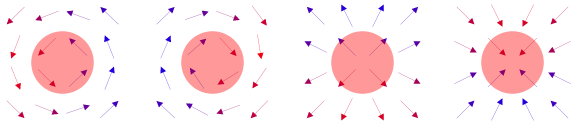
\includegraphics[width = 0.8\textwidth]{./vortices1.png}
\caption{Vortices, from left to right: center left, center right, source, sink}
\end{figure}

\begin{figure}[H]
\centering
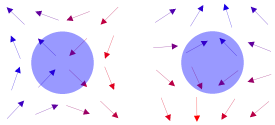
\includegraphics[width = 0.4\textwidth]{./vortices2.png}
\caption{Anti-vortices, both are saddles}
\end{figure}

\begin{figure}[H]
\centering
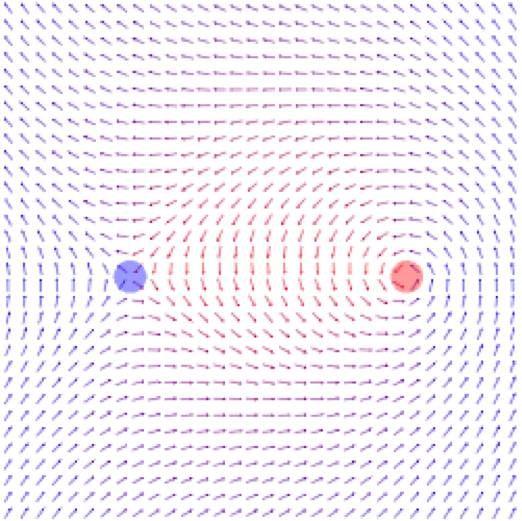
\includegraphics[width = 0.3\textwidth]{./vortex_pair.png}
\caption{a vortex pair}
\end{figure}

\section{Simulation Results}

\subsection{Observables}

My simulation is given for $J > 0$, which is the ferromagnetic case. The system size is from $8 \times 8$ to $64 \times 64$, with $2000$ steps to reach the thermal equilibrium. Then the calculation for the physical quantities is given with $20000$ steps after reaching the thermal equilibrium. So we can get the results as,

\begin{figure}[H]
\centering
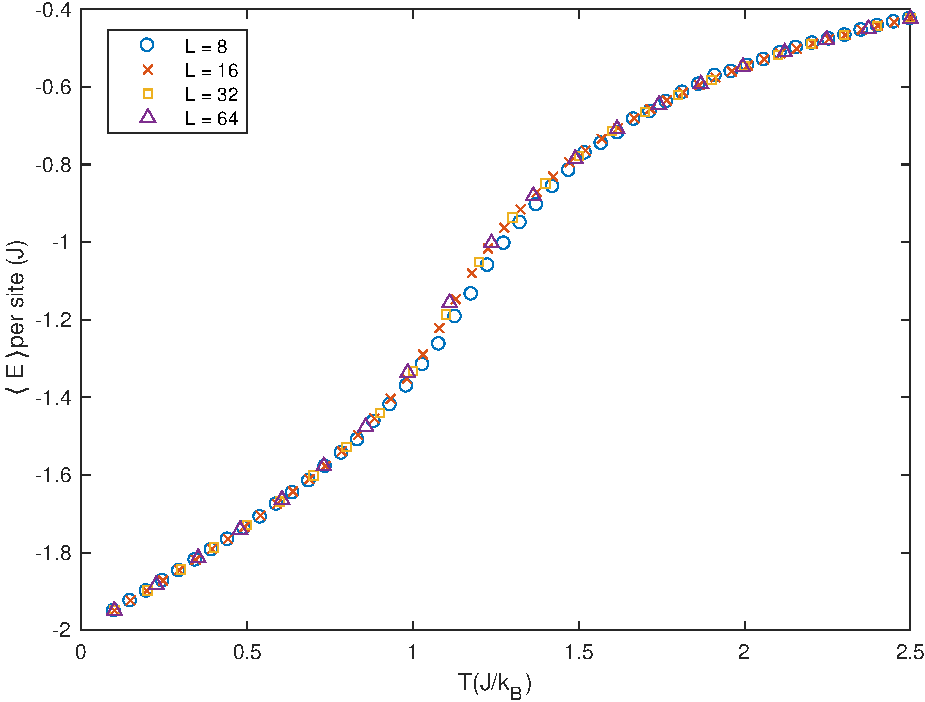
\includegraphics[width = 0.6\textwidth]{../Flux-Data/E_T-crop.pdf}
\caption{Energy Per Site}
\end{figure}

\begin{figure}[H]
\centering
\includegraphics[width = 0.6\textwidth]{../Flux-Data/CV_T-crop.pdf}
\caption{Specific Heat Per Site}
\end{figure}

The peak for $L = 64$ is not very clear above, so I pick this out as,

\begin{figure}[H]
\centering
\includegraphics[width = 0.6\textwidth]{../Flux-Data/CV_T_64-crop.pdf}
\caption{Specific Heat Per Site for $L = 64$}
\end{figure}

Then the other observables,

\begin{figure}[H]
\centering
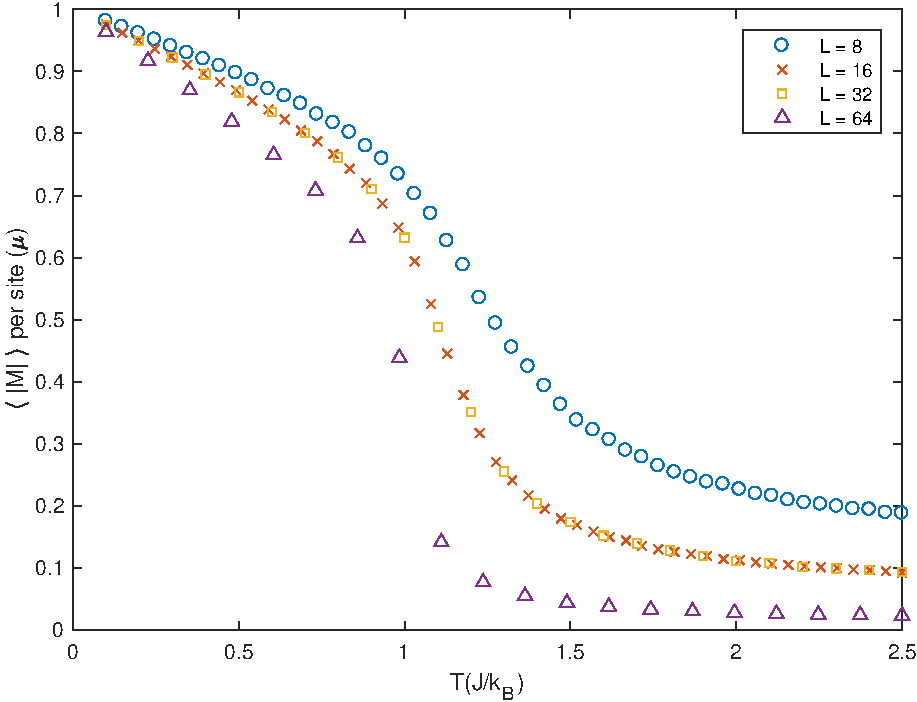
\includegraphics[width = 0.6\textwidth]{../Flux-Data/M_T-crop.pdf}
\caption{Abusolute Value of Magnetization Per Site}
\end{figure}

\begin{figure}[H]
\centering
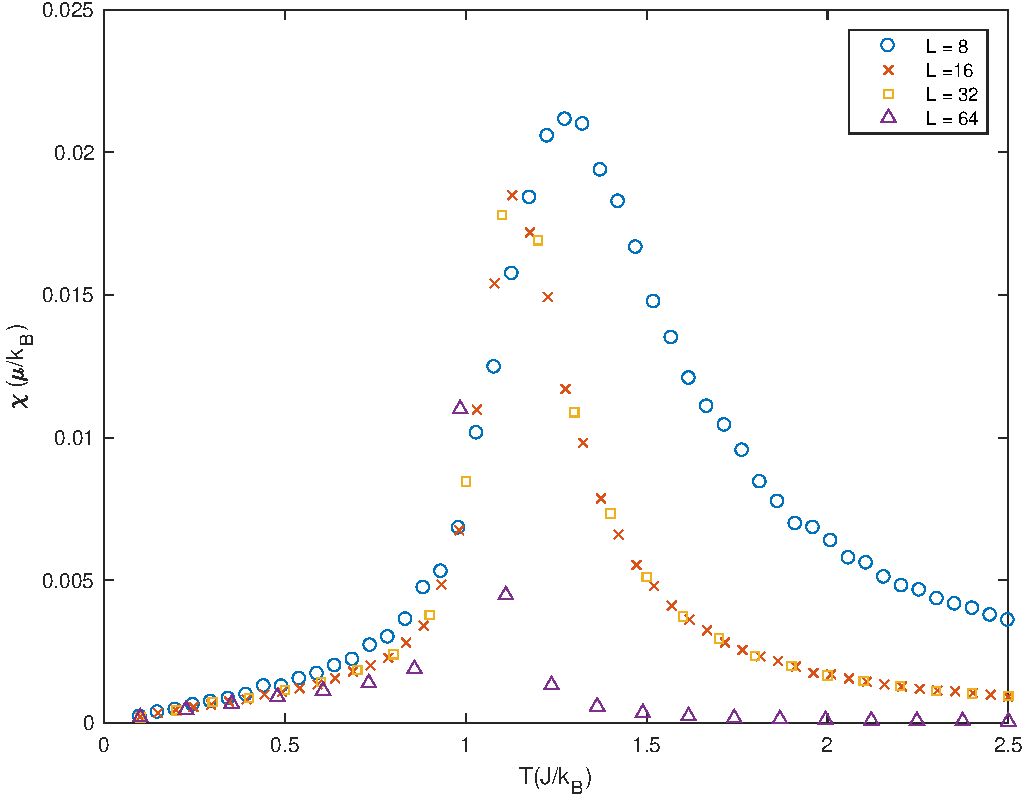
\includegraphics[width = 0.6\textwidth]{../Flux-Data/X_T-crop.pdf}
\caption{Magnetic Susceptibility Per Site}
\end{figure}

Clearly we can see KT phase transition since there is peak in $C_v$ and $\chi$ for XY spin system. Look at the finite size effect for the critical temperature $T_c$:

\begin{figure}[H]
\centering
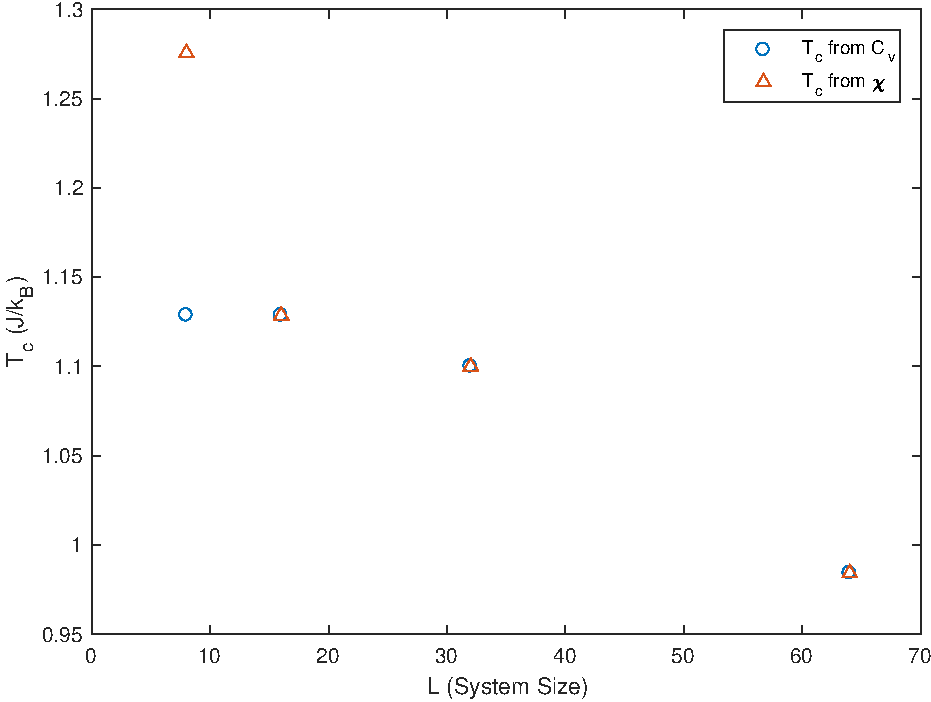
\includegraphics[width = 0.6\textwidth]{../Flux-Data/Tc_L-crop.pdf}
\caption{Finite Size Effect for $T_c$}
\end{figure}

So we can find the location of the phase transition approaches the limit for a infinitely large lattice: $T_c = 0.892 13(10) (\displaystyle \frac{J}{k_B})$\cite{olsson1995monte}. 

\subsection{Vortex}

Now look at the spin configurations after reaching the thermal equilibrium for the XY lattice system (System Size $L = 16$) and pick out the vortices (red) and anti-vortices (blue). The thermal equilibrium is got from $3000$ steps of Monte Carlo updates.

\begin{figure}[H]
\centering
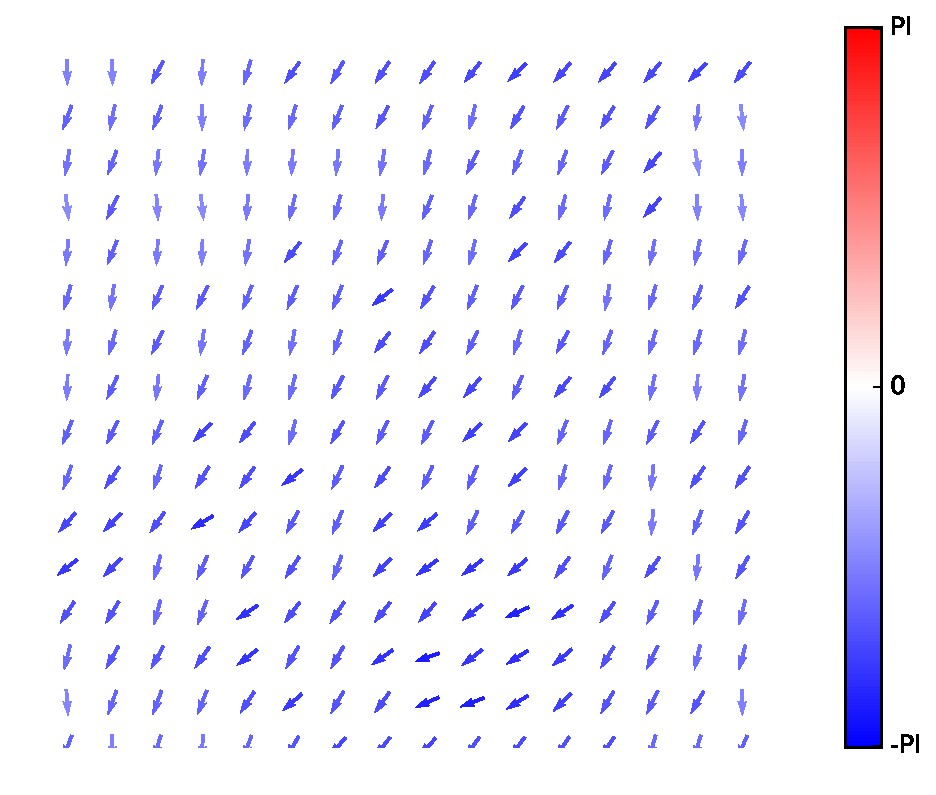
\includegraphics[width = 0.6\textwidth]{../vortex/XY-T0100.pdf}
\caption{Spin Configuration for $T = 0.10 (\displaystyle \frac{J}{k_B})$}
\end{figure}

\begin{figure}[H]
\centering
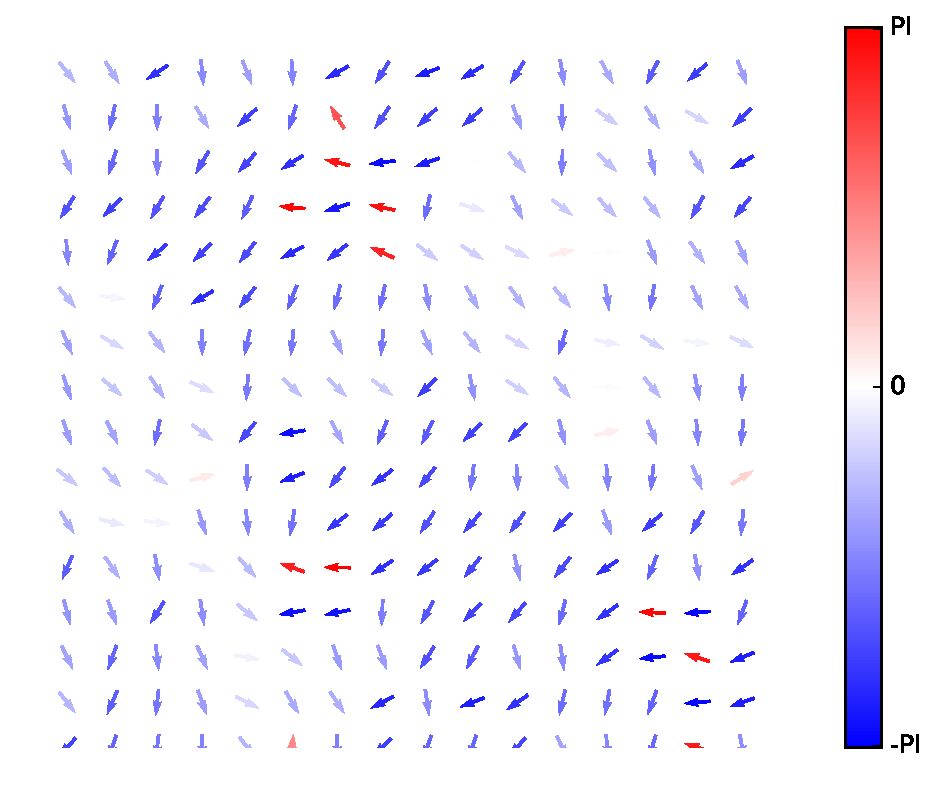
\includegraphics[width = 0.6\textwidth]{../vortex/XY-T0984.pdf}
\caption{Spin Configuration for $T = 0.98 (\displaystyle \frac{J}{k_B})$}
\end{figure}

\begin{figure}[H]
\centering
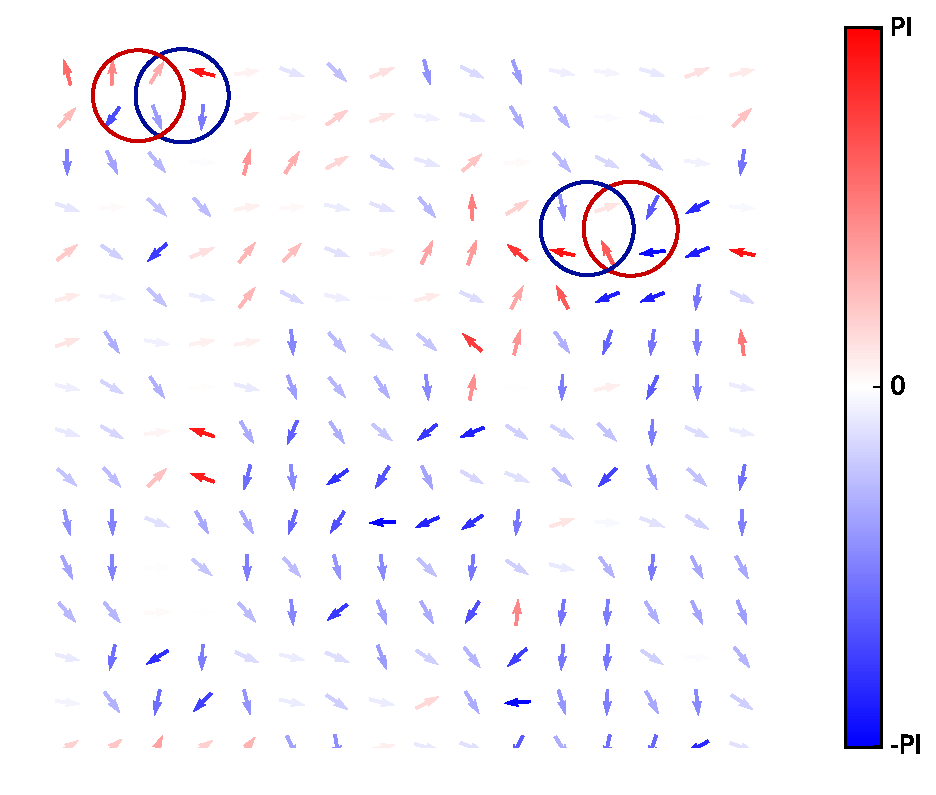
\includegraphics[width = 0.6\textwidth]{../vortex/XY-T1110.pdf}
\caption{Spin Configuration for $T = 1.11 (\displaystyle \frac{J}{k_B})$}
\end{figure}

So we can see that the vortex pairs are beginning to detach near critical temperature $T_c = 1.129 (\displaystyle \frac{J}{k_B})$ (For $L = 16$).

\begin{figure}[H]
\centering
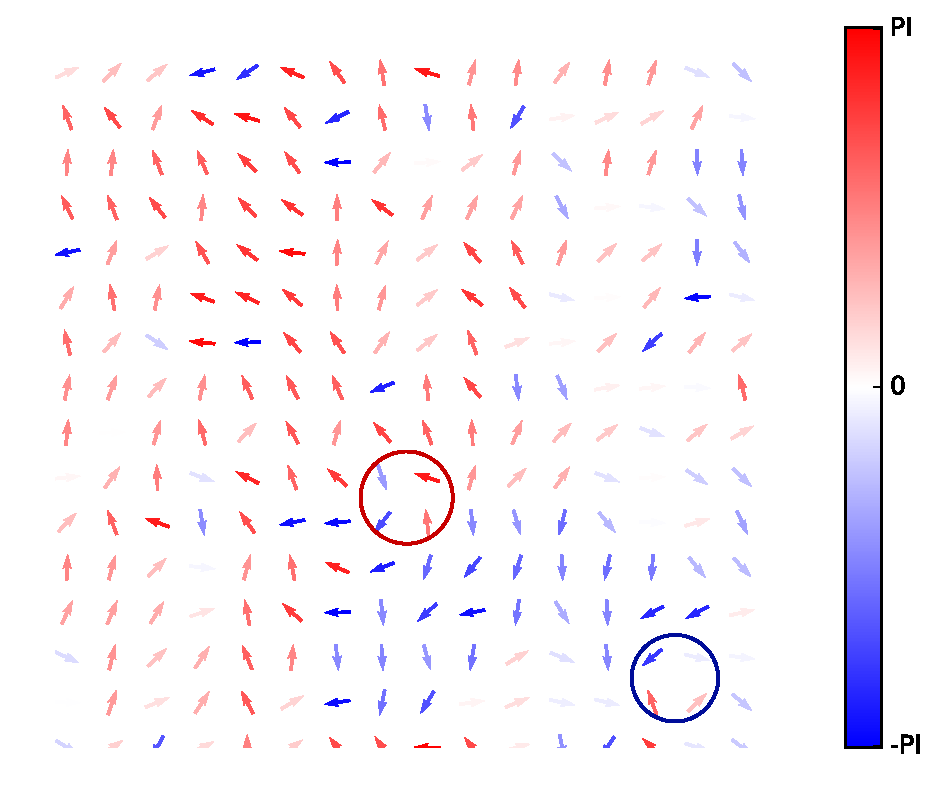
\includegraphics[width = 0.6\textwidth]{../vortex/XY-T1236.pdf}
\caption{Spin Configuration for $T = 1.24 (\displaystyle \frac{J}{k_B})$}
\end{figure}

\begin{figure}[H]
\centering
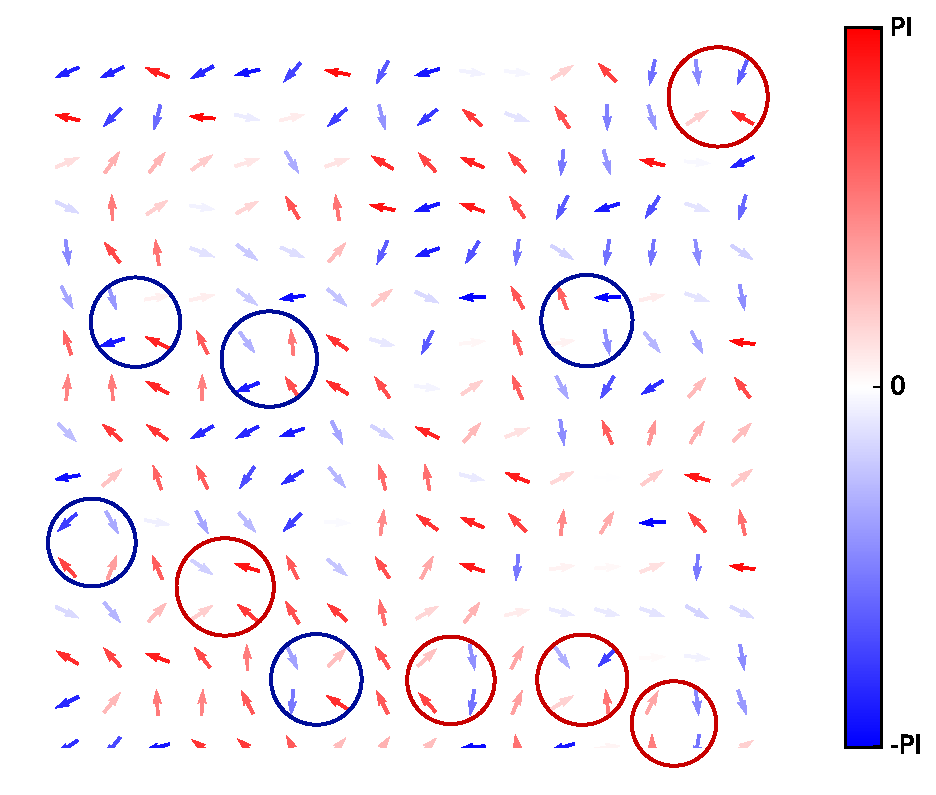
\includegraphics[width = 0.6\textwidth]{../vortex/XY-T2500.pdf}
\caption{Spin Configuration for $T = 2.50 (\displaystyle \frac{J}{k_B})$}
\end{figure}

From the peak in $C_v$, the critical temperature of this system size is $T_c = 1.129 (\displaystyle \frac{J}{k_B})$. Same temperature is gotten from $\chi$ in my simulation.

So when $T < T_c$, there are no vortices. When $T > T_c$, vortices begin to appear and usually they will appear in pairs. With the increase of the system temperature, the amount of vortices pairs is also increasing.

\section{Discussion}

\subsection{Mermin–Wagner Theorem}

The Mermin–Wagner theorem states that continuous symmetries cannot be spontaneously broken at finite temperature in systems with sufficiently short-range interactions in dimensions $d \leq 2$ \cite{mermin1966absence}. 

The 2-D XY model's KT phase transition is a special example for Mermin–Wagner theorem.

The Mermin–Wagner theorem prevents the 2-D XY model system to have any spontaneously symmetry broken. However, the KT phase transition is not associated with spontaneously symmetry broken. As a result, \textbf{Phase Transition} $\neq$ \textbf{Symmetry Breaking}.

Then Kosterlitz and Thouless proposed that topological defects could explain the phase transition. The 2-D XY system is not expected to have a second-order phase transition. However, one finds a low-temperature quasi-ordered phase with a correlation function that decreases with the distance like a power, which depends on the temperature. The transition from the high-temperature disordered phase with the exponential correlation to this low-temperature quasi-ordered phase is a Kosterlitz–Thouless transition. It is a phase transition of infinite order.

\bibliographystyle{unsrt}
\bibliography{FinalReport}  % list here all the bibliographies that
			     % you need. 

\section{Code}

\lstinputlisting{../KT-singleAxisProj.py}

\end{document}